\section{Introdução}

% Emoção/sentimentos/opiniões em arte.

Grande quantidade dos textos produzidos pelos seres humanos tem como
objetivo refletirem as opiniões e sentimentos do autor, em contraste
com a categoria de textos onde a preocupação é com fatos e expressões
objetivas. Dentro dos textos subjetivos, aqueles de cunho artístico sempre foram exemplo mais notável de expressividade emocional
\cite{PJA57}.

% Expressividade em música.

Uma das formas de arte mais antigas, a música consegue alcançar
níveis de expressividade emocional especialmente interessantes, 
combinando tanto a linguagem natural quanto sua própria linguagem
através de ritmo, sons, instrumentos, entre outros elementos. Sendo
dotada de tal capacidade de expressão, a música foi e continua
sendo estudada por cientistas da área da psicologia
\cite{juslin2001music} \cite{citeulike:12758145}
\cite{Aaltodoc:201705114245}. Dentre os 
vários aspectos que relacionam música e emoção, três deles são
particularmente instigantes para serem estudados:

\begin{itemize}
	\item Como emoções podem influenciar a música que alguém escolhe
	ouvir.
	\item Como música pode expressar emoção e sentimentos.
	\item Como música pode induzir emoções no ouvinte. 
\end{itemize}

\begin{figure}
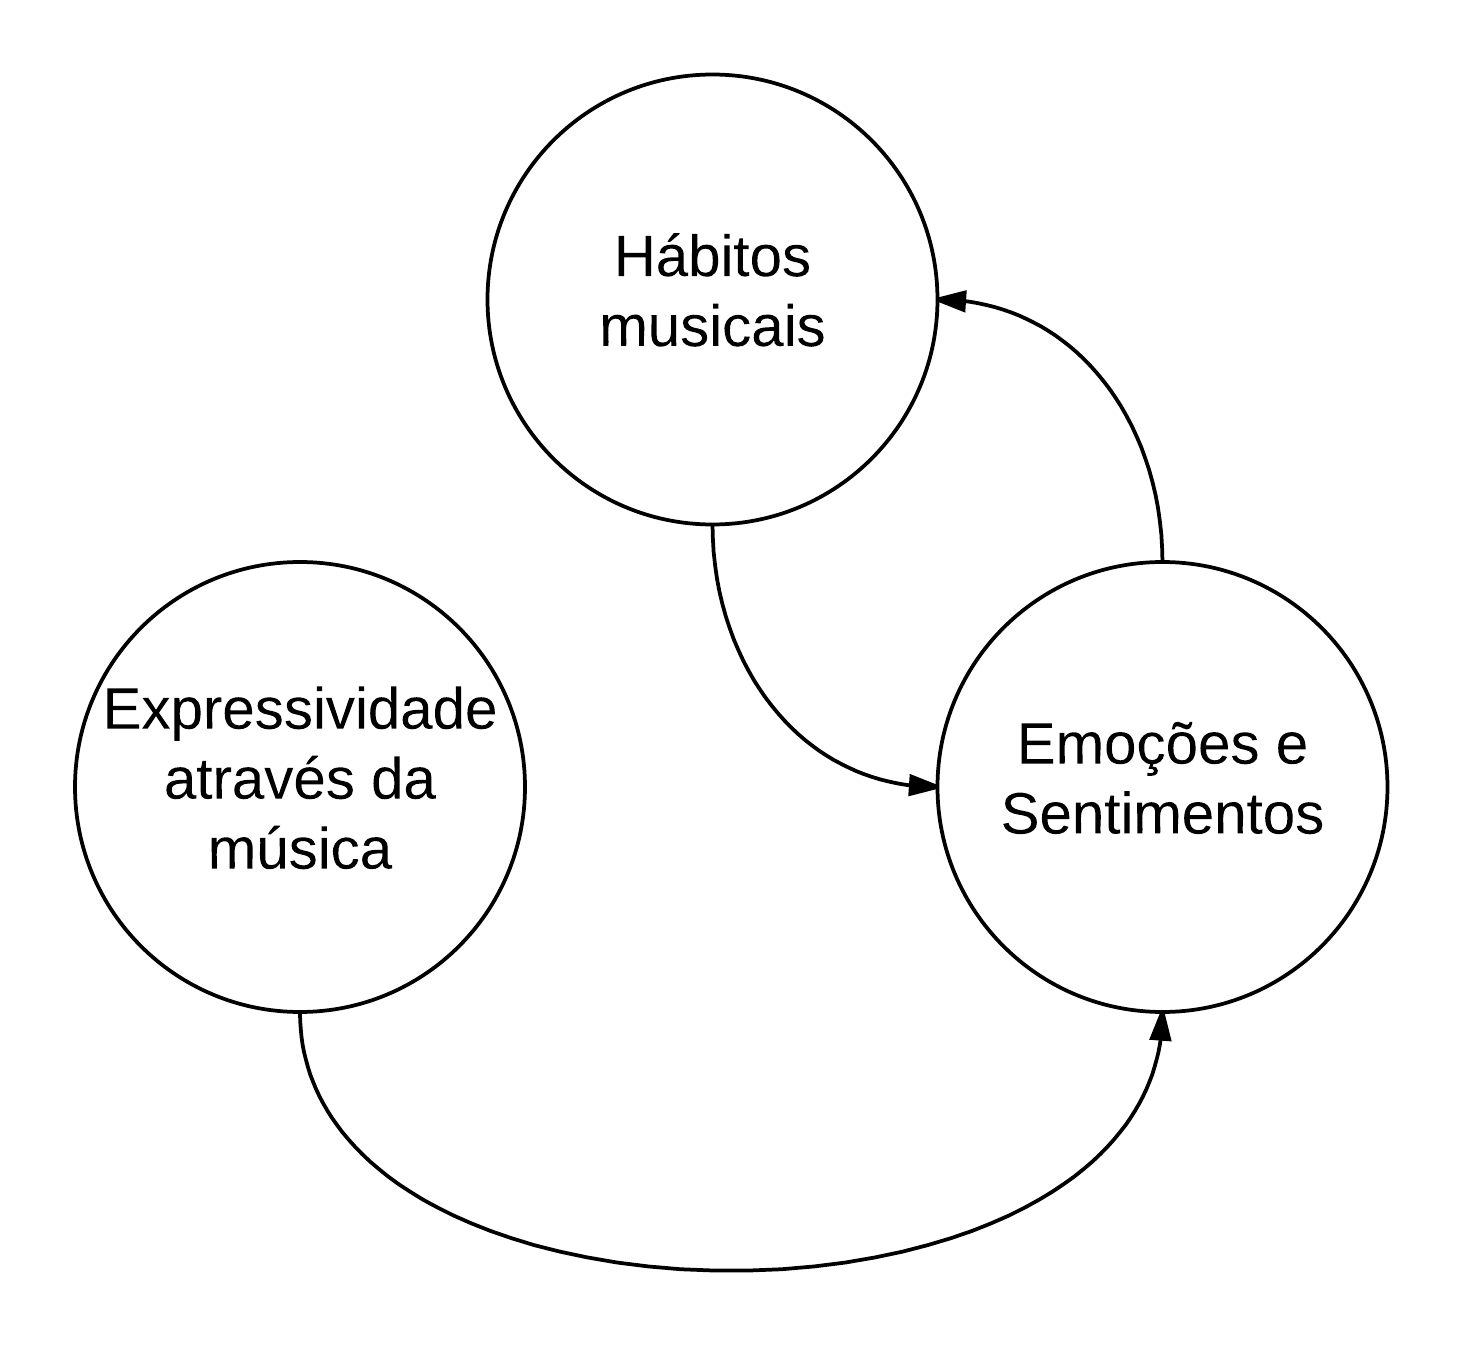
\includegraphics[height=3in, width=3in]{music-mood.png}
\caption{Relação entre expressividade de um artista através de sua música
	e o ciclo criado entre a indução de sentimentos no ouvinte e a escolha
	por músicas que correspondem a seu humor atual.}
\label{fig:music-mood}
\end{figure}

% Música como reflexo das emoções do ouvinte.
% Consumo massivo de música na modernidade - dados/estudo relevantes.
Já sabemos que os hábitos musicais de uma pessoa influenciam diretamente
seu humor, sentimentos e emoções \cite{mccraty1998}. Mais especificamente, existem estudos que demonstram a influência das letras
de uma música no humor e comportamento do ouvinte
\cite{doi:10.2190/35T0-U4DT-N09Q-LQHW}. Esses dois aspectos, aliados
 ao fato de que o consumo de música sofreu grande aumento com a chegada
 das plataformas de streaming digital e compartilhamento de arquivos
 \cite{doi11044343huang} nos fornecem grande indicação
  de que podemos utilizar os hábitos musicais de um ouvinte como fonte de
 informações a respeito do humor e emoções do mesmo.

\section{Problema}

Diante da relação íntima entre humor e hábitos musicais, uma tarefa
particularmente relevante é aquela de identificar usuários (ouvintes)
cujos hábitos de consumo musical denotam possíveis transtornos
psicológicos e de humor. Enquanto esse tipo de análise é muito simplista
para determinar qualquer tipo de transtorno com acurácia, ele pode servir
como um forte indicador de alterações de humor e, como tal, identificador
de usuários que necessitam de algum tipo de suporte emocional.

Plataformas de streaming e recomendação de música online como Last.fm
\cite{haupt2009} e Spotify \cite{5569963}
possuem bases de dados massivas sobre seus usuários
\cite{pichl2014combining} \cite{4736778}, contendo informações
sobre seus artistas favoritos, músicas, álbuns, além de coletar, em tempo
real, informações sobre o hábito musical de um ouvinte. Dessa forma,
essas plataformas a base de dados ideal para a tarefa de identificar 
o humor de um usuário baseado nas músicas que este ouve.

A partir desses dados, é possível coletar os hábitos musicais de um
determinado usuário ao longo de um intervalo de tempo qualquer. Com
esses dados em mão e uma abordagem que envolve tanto os campos de
processamento de linguagem natural - mais especificamente a área
de análise de sentimentos, para tentar posicionar as letras de uma música 
no espectro de emoções humanas -, quanto a área da psicologia e música
em si, podemos tentar extrair, a partir dos hábitos musicais de um
usuário, suas emoções e sentimentos, identificando em último caso aqueles
que demonstram maior necessidade de intervenção e suporte psicológico, 
que pode ser oferecido de várias maneiras diferentes pelas próprias
plataformas.

\section{Modelagem} \label{sec:mod}

% Coleta de dados
O primeiro passo para resolver abordar esse problema é determinar como coletar os dados necessários para traçar um panorama sobre os hábitos
musicais de um usuário. Para isso, a plataforma Last.fm foi escolhida,
não só pela quantidade massiva de dados que acumula, mas também pelo
fato de que todos os seus dados são exibidos publicamente na mesma,
como definido nos termos de contrato do serviço \cite{Lastfmterms}.

% Parâmetros
Nessa etapa é importante definir a quantidade $ n $ para determinar
 as últimas $ n $ músicas que um usuário ouviu. Essa não é uma escolha
 muito simples, uma vez que, para valores muito altos de $ n $, perdemos
 acurácia, no sentido de que essas músicas podem refletir um período de
 tempo muito longo, onde as emoções do usuário podem variado 
 arbitrariamente. Por outro lado, é desejável escolher um valor de $ n $
 suficientemente alto para reunir a maior quantidade possível de músicas
 que refletem um mesmo estado de sentimento/humor do usuário.

% Letras
Em seguida, é preciso reunir os atributos das canções que servirão de 
indicadores para as emoções das mesmas e, consequentemente, dos usuários.
O primeiro atributo a ser considerado são as letras das músicas. Para 
facilitar a implementação do trabalho, só foram levadas em consideração
letras das músicas cujo idioma é o inglês (uma vez que já existe uma grande
quantidade de ferramentas existentes para trabalhar com esse idioma).

De posse das letras de uma canção, podemos tentar quantificar a negatividade
das palavras. Para isso, podemos usar uma base de dados que já contenha
emoções associadas a cada palavra. Para esse trabalho, foi escolhida
a base \textit{NRC Word-Emotion Association Lexicon}
\cite{Mohammad13}. Além disso, é necessário realizar um pré-processamento
no texto, removendo as flexões das palavras e excluindo aquelas cuja
classe gramatical não seja forte indicador de sentimento ou emoção, i.e.,
palavras como 'hi', 'him', 'there', etc. Com isso, conseguimos quantificar
a porcentagem de palavras negativas nas letras de uma música, onde uma
palavra é considerada negativa se, no lexicon de referência, ela ativa
sentimentos considerados negativos como raiva e medo.

Um fator importante a ser considerado para a análise das letras de uma canção
diz respeito ao peso ou densidade das letras em relação à canção como um todo.
Isto é, é importante verificar o quanto o humor de uma canção é influenciado
pelas suas letras. Imaginemos o caso de uma música de duração de 10 minutos. 
Caso essa canção possua apenas duas frases ao longo dos 10 minutos, é natural
pensar que essas duas frases terão pouco impacto no humor geral da canção, ao
passo que, caso ao longo dos 10 minutos haja poucos intervalos sem qualquer
letra, então podemos pensar que o humor dessa canção é fortemente 
influenciada por suas letras. A partir disso, definimos o conceito de 
\textit{peso lírico}, que se refere a quão alto é o fluxo lírico em uma canção
por segundo de duração.

% Músicas instrumentais
Naturalmente, canções instrumentais também devem ser identificadas
e tratadas de forma especial, de modo que também possam ser extraídas 
informações importantes das mesmas. De fato, o essas canções recebem no
trabalho o mesmo tratamento de canções cujo idioma é diferente do inglês,
uma vez que a análise da letra dessas também não foi incluída, como
mencionado anteriormente.

% Valência
Para uma análise mais razoável e completa, é necessário obter uma medida de
negatividade para as canções instrumentais e aquelas cujas letras não podem
ser analisadas. Para isso, a decisão foi de incluir uma medida já definida
pela própria plataforma de streaming Spotify \cite{spotifyvalence}, chamada
valência (\textit{valence}). De acordo com a própria documentação da API do
Spotify, essa medida é definida como:

\begin{quote}
	Uma medida de 0.0 a 1.0 que descreve a positividade musical transmitida
	por uma faixa. Faixas com valência alta soam mais positivas (e.g. felizes,
	alegres, eufóricas), enquanto faixas com baixa valência soam mais
	negativas (e.g. tristes, deprimentes, irritadas). - (tradução livre)
\end{quote}

Dessa forma, temos três medidas para construir o índice de negatividade de
uma canção, seu peso lírico, a negatividade lírica e a valência. Essas três
medidas serão usadas para definir o índice de negatividade de cada canção
que um determinado usuário ouviu ao longo do tempo, obtendo-se assim uma
medida indicadora do próprio humor do usuário.

\section{Implementação}

Nessa seção são discutidas todas as decisões de implementação tomadas
durante o desenvolvimento do trabalho em questão.

\subsection{Linguagem e Bibliotecas}

A partir da modelagem descrita na Seção \ref{sec:mod}, foi desenvolvida
uma ferramenta para análise dos sentimentos de um usuário através de seus
hábitos musicais. A ferramenta foi apelidada de \textit{Moodic} (um jogo
de palavras com \textit{mood} e \textit{music} - humor e música em inglês).

A ferramenta foi desenvolvida utilizando a linguagem Python 3 \cite{python3}.
Essa linguagem foi escolhida pela grande quantidade de ferramentas para
processamento de linguagem natural disponíveis para uso gratuito através da
mesma.

Para a coleta de letras das canções, por exemplo, foi utilizada a biblioteca
\textit{lyricwikia} \cite{lyricwikia}. Para essa tarefa, não houve qualquer
fator decisivo na escolha, porém o ideal, para trabalhos futuros, seria
a escolha de uma biblioteca com o maior banco de dados possível, a fim
de evitar que um grande número de canções, mesmo aquelas que possuem letras,
não tenham suas letras encontradas pelo programa e, como tal, acabem sem
uma medida de negatividade lírica.

Com relação à coleta de dados da plataforma Last.fm, foi identificado um
\textit{wrapper} em Python para a própria API da plataforma. Essa biblioteca,
a \textit{pyLast} \cite{pylast} fornece acesso aos dados da plataforma de
forma fácil, com ela, é possível coletar dados sobre canções, álbuns e
músicas escutadas por um determinado usuário. Para esse trabalho, somente
foi necessária a utilização da mesma para coletar as $ n $ canções ouvidas
por um usuário.

De forma similar, a biblioteca \textit{Spotipy} \cite{spotipy} fornece uma
interface em Python para a API Web da plataforma Spotify. Com essa biblioteca,
o programador consegue obter os dados de um artista, canções, álbuns, imagens,
etc. O interesse para o trabalho em questão, entretanto, é obter algumas
informações interessantes sobre as faixas ouvidas por um usuário, como
duração (necessária para o cálculo de peso lírico) e valência.

Também é importante mencionar a biblioteca \textit{langdetect}
\cite{langdetect}, que foi responsável por detectar a linguagem de cada uma
das letras das músicas, permitindo que o programa apenas trabalhasse com
letras em inglês.

Por fim, a biblioteca \textit{NLTK} \cite{Perkins:1953497} foi de grande utilidade para realizar o pré-processamento do texto das canções, como
descrito na Seção \ref{subsec:pre}, além da tarefa de filtragem das
palavras cujas classes gramaticais eram mais relevantes para o programa,
como descrito na Seção \ref{subsec:pos}.

\subsection{NRC Word-Emotion Association Lexicon} \label{subsec:nrc}

O processo de quantificação de negatividade nas letras de uma determinada
canção começa no problema de como associar emoções a palavras. Há várias
abordagens que podem ser utilizadas nesse problema, seja levando em 
consideração palavras individualmente ou sentenças de $ k $ palavras. 
A fim de facilitar implementação, a escolha para esse trabalho foi a de
analisar cada palavra do texto de uma música de forma individual, isto é,
sem considerar as palavras que cercam uma determinada palavra (seu contexto).

Para isso, foi utilizado o NRC Emolex, que consiste em uma grande lista de
palavras, seguidas de 10 possíveis emoções, seguidas de um número (0 ou 1),
que indica se aquela palavra "ativa" tal emoção ou não, sendo 0 representante
de emoção não ativada e 1 de emoções ativadas. O conceito de ativação aqui
indica simplesmente associação entre a palavra e a emoção que transmite, de 
forma isolada, sem informações de contexto.

\begin{table}[h]
	\centering
	\begin{tabular}{|c|c|c|}
		\hline
		\textbf{Palavra} & \textbf{Emoção} & \textbf{Ativação} \\ \hline
		suicide & anger & 1 \\ \hline
		suicide & anticipation & 0 \\ \hline
		suicide & disgust & 0 \\ \hline
		suicide & fear & 1 \\ \hline
		suicide & joy & 0 \\ \hline
		suicide & negative & 1 \\ \hline
		suicide & positive & 0 \\ \hline
		suicide & sadness & 1 \\ \hline
		suicide & surprise & 0 \\ \hline
		suicide & trust & 0 \\ \hline
	\end{tabular}
	\caption{\label{tab:emolexword} Exemplo de dados do NRC Emolex para a 
	palavra "suicide".}
\end{table}

\subsection{Emoções negativas}

Através do lexicon apresentado na Seção \ref{subsec:nrc}, foi necessário
definir quais dentre as 10 emoções teriam influência no índice de 
negatividade de uma canção. De maneira geral, as 10 emoções presentes 
no lexicon são muito bem definidas como negativas ou positivas, sendo
a separação feita como mostrado na Tabela \ref{tab:emolexposneg}.

\begin{table}[h]
	\centering
	\begin{tabular}{|l|p{20mm}|}
		\hline
		\textbf{Polaridade} & \textbf{Emoções} \\ \hline
		Positivo & Joy \newline Trust \\ \hline
		Neutro & Anticipation \newline Surprise \\ \hline
		Negativo & Anger \newline Disgust \newline Fear 
		\newline Negative \newline Sadness \\ \hline
	\end{tabular}
	\caption{\label{tab:emolexposneg} Separação das emoções do NRC Emolex em
	positivas e negativas.}
\end{table}

Após essa separação de polaridades, o foco do trabalho foi nas emoções
negativas. Dessa forma, ao processar uma palavra no texto de uma canção,
o programa verifica se a mesma ativa alguma das emoções negativas,
como definido na Tabela \ref{tab:emolexposneg}. Caso isso aconteça,
um contador de palavras negativas é incrementado.

Essa abordagem é simplista e poderia ser melhorada para incluir pesos
às diferentes emoções dentro da polaridade negativa. Por exemplo, poderia
ser interessante definir que a emoção \textit{disgust} é mais
\textit{anger}, ou vice-versa. Essas decisões devem levar em conta o propósito da aplicação. Para o trabalho em questão, como o objetivo é
simplesmente determinar um índice de negatividade, a abordagem não
levou em consideração pesos.

\subsection{Pré-processamento de texto} \label{subsec:pre}

Uma tarefa fundamental em processamento de linguagem natural diz respeito 
ao pré-processamento do texto a ser analisado, uma vez que esse, em sua 
maioria, não se apresenta de forma estruturada, isto é, com o formato
necessário para ser usado como entrada para os diversos algoritmos existentes
\cite{Manning:1999:FSN:311445}.

Para o trabalho em questão, foi necessário coletar as letras das canções em 
formato bruto e transformá-las em uma lista de palavras no mesmo formato em
que se apresentam as palavras no NRC Emolex. Para isso, o primeiro passo
foi realizar um processo de \textit{tokenização} onde a letra de uma canção,
inicialmente uma longa string, é quebrada em tokens. Para cada um desses
tokens, aplicamos um algoritmo de \textit{lematização}, removendo flexões.

Cada token também foi transformado em seu equivalente apenas com letras
minúsculas. Além disso, é importante remover do texto original aqueles tokens que não representam palavras. Esses podem ser tanto numerais quanto símbolos de pontuação. Por fim, foram removidas do texto aquelas palavras que denotam
conectores sentenciais, como "if", "into", "in", etc, uma vez que essas
palavras não denotam emoções e, portanto, não são relevantes para a nossa
análise.

\begin{figure}
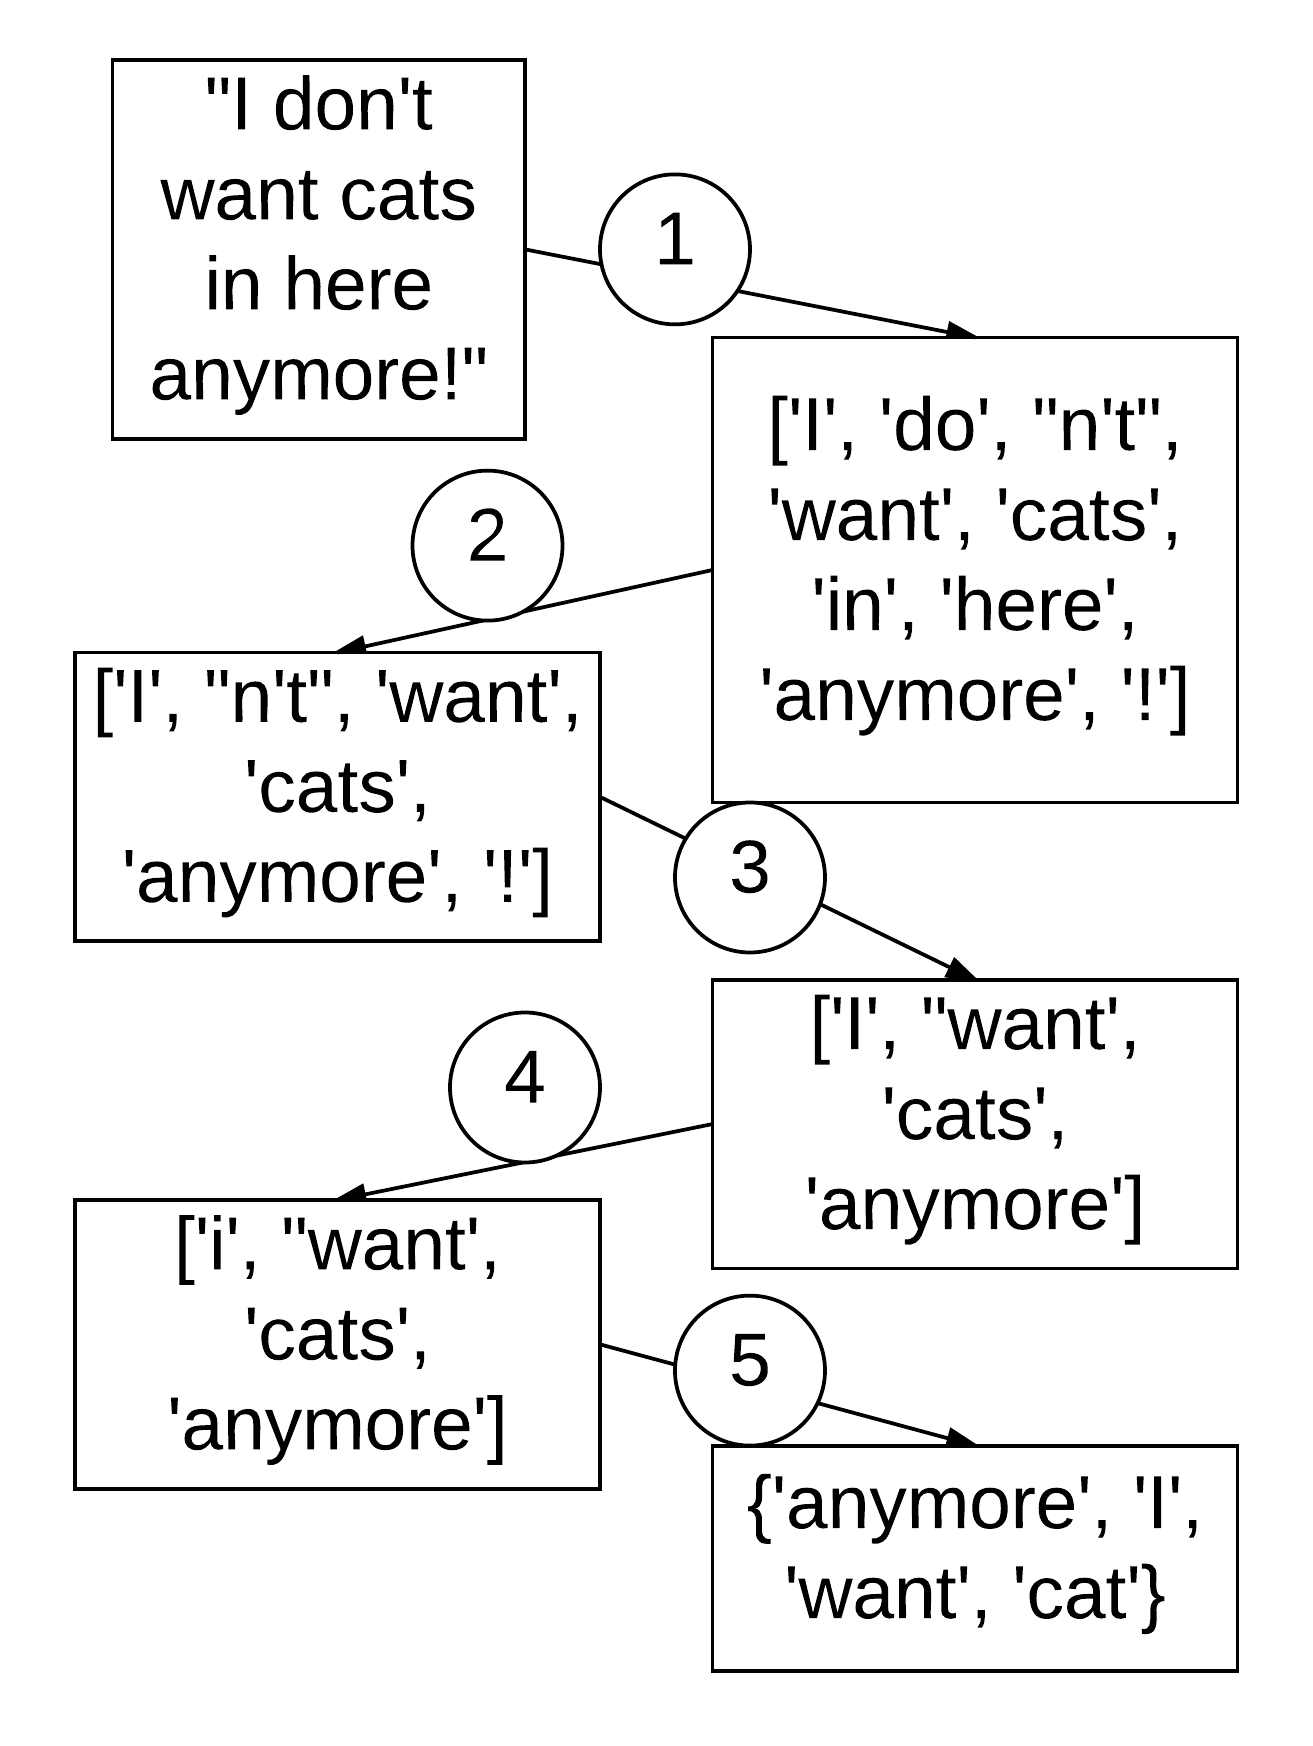
\includegraphics[height=4in, width=3in]{textpre.png}
\caption{Pré-processamento de texto realizado para cada texto de canção
encontrada pelo programa. 1: A string que se refere à letra de uma canção
é quebrada em tokens. 2: Remove-se conectores sentenciais dos tokens.
3: Remove-se tokens não formados exclusivamente por letras. 4:
Todas as letras dos tokens são transformadas para minúsculas. 
5: Remove-se as flexões dos tokens. Observamos que o token "i" volta 
a apresentar letras maiúsculas. Isso se deve ao fato de que a palavra
"I" inglês sempre tem grafia em maiúsculo.}
\label{fig:music-mood}
\end{figure}

\subsection{Classes gramaticais não expressivas} \label{subsec:pos}

Um fator importante observado durante a implementação do trabalho foi o de
que o NRC Emolex contém somente determinados tipos de palavras. Esses tipos
são definidos pelas suas classes gramaticais. Logo, foi importante filtrar
dos tokens obtidos através das letras de uma canção aqueles cuja classe
gramatical não faça parte do Emolex. Com isso, aumentamos a precisão da 
análise que conta as palavras negativas no conjunto de tokens. 

Essa filtragem que mantém apenas as classes gramaticais emocionalmente
expressivas foi feita de forma empírica, observando, de todas as classes
gramaticais possíveis dentro da biblioteca NLTK, aquelas que não indicam
necessariamente algum tipo de humor ou sentimento. A lista das classes
gramaticais definidas como não expressivas é apresentada na Tabela
\ref{tab:nonexppos}.

\begin{table}[h]
	\centering
	\begin{tabular}{|c|c|}
		\hline
		\textbf{Classe Gramatical na NLTK} & \textbf{Descrição} \\ \hline
		CC & Conjunção coordenativa \\ \hline
		CD & Dígito cardinal \\ \hline
		DT & Determinador \\ \hline
		EX & "There" existencial: "there is" \\ \hline
		IN & Preposição / Conjunção subordinativa \\ \hline
		LS & Marcador de lista: 1) \\ \hline
		NNP & Nome próprio \\ \hline
		POS & Terminações possessivas: parent's \\ \hline
		PRP & Pronome pessoal \\ \hline
		PRP\$ & Pronome possessivo \\ \hline
		TO & "To" quando usado como preposição \\ \hline
		UH & Interjeições \\ \hline
		WDT & Determinador wh: "which" \\ \hline
		WP & Pronomes wh: "who", "what" \\ \hline
		WP\$ & Pronome possessivo wh: "whose" \\ \hline
		WRB & Advérbios wh: "where", "when" \\ \hline
	\end{tabular}
	\caption{\label{tab:nonexppos} Relação das classes gramaticais na
	biblioteca NLTK definidas como não expressivas emocionalmente no
	NRC Emolex.}
\end{table}

\subsection{Peso lírico}



\subsection{Índice de negatividade}

\section{Estudo de caso}



\section{Conclusão}

% Sugestões futuras
	% Ampliar as linguagens suportadas
	% Dar peso para diferentes emoções
	% O que pode ser feito com os dados obtidos
